\documentclass[nohyper,justified]{tufte-handout}\usepackage[]{graphicx}\usepackage[]{color}
%% maxwidth is the original width if it is less than linewidth
%% otherwise use linewidth (to make sure the graphics do not exceed the margin)
\makeatletter
\def\maxwidth{ %
  \ifdim\Gin@nat@width>\linewidth
    \linewidth
  \else
    \Gin@nat@width
  \fi
}
\makeatother

\definecolor{fgcolor}{rgb}{0.345, 0.345, 0.345}
\newcommand{\hlnum}[1]{\textcolor[rgb]{0.686,0.059,0.569}{#1}}%
\newcommand{\hlstr}[1]{\textcolor[rgb]{0.192,0.494,0.8}{#1}}%
\newcommand{\hlcom}[1]{\textcolor[rgb]{0.678,0.584,0.686}{\textit{#1}}}%
\newcommand{\hlopt}[1]{\textcolor[rgb]{0,0,0}{#1}}%
\newcommand{\hlstd}[1]{\textcolor[rgb]{0.345,0.345,0.345}{#1}}%
\newcommand{\hlkwa}[1]{\textcolor[rgb]{0.161,0.373,0.58}{\textbf{#1}}}%
\newcommand{\hlkwb}[1]{\textcolor[rgb]{0.69,0.353,0.396}{#1}}%
\newcommand{\hlkwc}[1]{\textcolor[rgb]{0.333,0.667,0.333}{#1}}%
\newcommand{\hlkwd}[1]{\textcolor[rgb]{0.737,0.353,0.396}{\textbf{#1}}}%

\usepackage{framed}
\makeatletter
\newenvironment{kframe}{%
 \def\at@end@of@kframe{}%
 \ifinner\ifhmode%
  \def\at@end@of@kframe{\end{minipage}}%
  \begin{minipage}{\columnwidth}%
 \fi\fi%
 \def\FrameCommand##1{\hskip\@totalleftmargin \hskip-\fboxsep
 \colorbox{shadecolor}{##1}\hskip-\fboxsep
     % There is no \\@totalrightmargin, so:
     \hskip-\linewidth \hskip-\@totalleftmargin \hskip\columnwidth}%
 \MakeFramed {\advance\hsize-\width
   \@totalleftmargin\z@ \linewidth\hsize
   \@setminipage}}%
 {\par\unskip\endMakeFramed%
 \at@end@of@kframe}
\makeatother

\definecolor{shadecolor}{rgb}{.97, .97, .97}
\definecolor{messagecolor}{rgb}{0, 0, 0}
\definecolor{warningcolor}{rgb}{1, 0, 1}
\definecolor{errorcolor}{rgb}{1, 0, 0}
\newenvironment{knitrout}{}{} % an empty environment to be redefined in TeX

\usepackage{alltt}
\usepackage{mathtools}
%%\usepackage{marginnote}
%%\usepackage[top=1in, bottom=1in, outer=5.5in, inner=1in, heightrounded, marginparwidth=1in, marginparsep=1in]{geometry}
\usepackage{enumerate}
%% mess with the fonts
%%\usepackage{fontspec}
%%\defaultfontfeatures{Ligatures=TeX} % To support LaTeX quoting style
\usepackage[T1]{fontenc}
\usepackage[utf8]{inputenc}
% For package xtable
\usepackage{booktabs}  % Nice toprules and bottomrules
\heavyrulewidth=1.5pt  % Change the default to heavier lines
%%\usepackage{longtable} 
%%\usepackage{tabularx}  % To control the width of the table

% this should make caption font bold.
%%\usepackage{xstring}
%%\usepackage{etoolbox}

%%\usepackage{url}

%% xetex only \usepackage{breakurl}
\usepackage{float} % for fig.pos='H'
%%\usepackage{wrapfig}
%%\usepackage{tikz}


\usepackage{colortbl,xcolor}

\makeatletter
\title{Introduction to Data Analysis}
\author{Kate Davis}
\makeatother

\newcommand{\dev}[1] {Dev_{\bar{#1}}}
\IfFileExists{upquote.sty}{\usepackage{upquote}}{}
\begin{document}




\maketitle
\section{Introduction to Data Analysis}
Statistical Data Analysis is quantitative evaluation of \textbf{Numeric Data}\marginnote{\textbf{Numeric Data} points are numbers that represents value. Generally, each numeric data point  has a unit of measure} and multiple data points with the same unit can be combined using basic arithmetic operations to form a new data point. Height (in mm), weight (in kg), temperature (degrees F), proportions (percent), and monetary values are examples of  \textbf{continuous}\marginnote{\textbf{Continuous Data} has an infinite number of possible values within a given range, usually represented by real numbers, percentages or fractions} numeric data points. \textbf{Discrete}\marginnote{\textbf{Discrete Data} are data with a finite list of possible values within any given range, and are often integer or count data} numeric data are whole number data or count data, such as the number of sunspots per month, the number of apples in a bushel, or dice roll values.  House numbers, credit scores, zipcodes and jersey numbers are examples of numbers that are not numeric data points, as none have units nor can these numbers be combined arithmetically to form another numeric data point.

\section{Height in Whole Inches}
Consider the numeric \textbf{Data Set}\marginnote{A \textbf{Data Set} is a collection of numeric data points. Each data point within a data set is called an observation, denoted $x_i$, where $i$ is the number of the observation. For our data set, $x_3$ is 72. $N$ denotes the number of observations.} of \textbf{Height in Whole Inches} of our \textbf{Population}\marginnote{A \textbf{Population} is any complete group or set of measure with at least one characteristic in common}: students in MA3200 Section 2. Heights would be continuous data, but we have ``discretized'' this data by rounding to the nearest whole inch. The data, in the original order presented, is:

\begin{knitrout}
\definecolor{shadecolor}{rgb}{0.969, 0.969, 0.969}\color{fgcolor}\begin{kframe}
\begin{verbatim}
64 70 72 73 69 67 68 66 62 71 66 72 67 74
71 72 67 71 65 65 69 71 69 72 71 68 63 64
\end{verbatim}
\end{kframe}
\end{knitrout}
This set of data has 28 data points. To better evaluate this data, lets sort it. We can begin to see patterns of multiple values, and can quickly see that the lowest or minimum value is 62 inches and the highest or maximum value is 74 inches. The \textbf{Range}\marginnote{The \textbf{Range} is difference between the maximum and minimum values of a data set} is 12 inches.

\begin{knitrout}
\definecolor{shadecolor}{rgb}{0.969, 0.969, 0.969}\color{fgcolor}\begin{kframe}
\begin{verbatim}
62 63 64 64 65 65 66 66 67 67 67 68 68 69
69 69 70 71 71 71 71 71 72 72 72 72 73 74
\end{verbatim}
\end{kframe}
\end{knitrout}

This data set has 13 discrete values for height, fewer than the range of 12 inches. There is a gap in observations between 62 inches and 74 inches, but all other height values in the range are represented.

To gain more knowledge about this dataset, we must describe the \textbf{distribution}\marginnote{The Oxford English Dictionary defines \textbf{Distribution} as the \emph{way in which something is shared out among a group or spread over an area} } of values across the measurement range, with a goal of using that information for predictions, estimations and other inferences about the population when a complete \textbf{census}\marginnote{A \textbf{Census} is a complete enumeration of every unit, everyone or everything in a population.} 

The \textbf{statistical distribution}\marginnote{A \textbf{Statistical Distribution} assigns probabilities to the possible values of a data set } can be estimated or inferred from a data set, and 
is used to estimate the accuracy of these predictions, estimates, inferences.

\section{Frequency Tables}
We can create a \textbf{Frequency table}\marginnote{a \textbf{Frequency Table} is a summary of data point Frequency by class or interval} and \textbf{histogram}\marginnote{a \textbf{Histogram} is a chart that displays the distribution of a data set} of the data set values. The height data is in whole inches, so we will start with using the integer height value as the class in integer order. A cumulative frequency column is added for additional calculation.



\section{Measures of Center}


To understand more about the distribution of the height in inches of our studens, we first examine ``centers'' of the data: the mode, the median, and the mean.

The \textbf{mode}\marginnote{The \textbf{Mode} of a data set is value that has the highest frequency} of this dataset is 71 inches with frequency 5 students. The mode is easily found from the frequency table. If there is one clear mode in a distribution, the dataset is said to be \emph{unimodal}. A data set can have more than one mode, or be \emph{multi-modal}.

The \textbf{median}\marginnote{The \textbf{Median} of a data set is the midpoint of the distribution, or the middle value of the data when sorted in ascending order. The median is the 50th percentile} of this dataset is 69 inches with frequency of NA students. If the number $n$ of data points is odd, this is a simple observation of $(n+1)/2$. If the number of data points is even, the arithmetic average of the nearest two data point values is the median.

The \textbf{mean}\marginnote{The \textbf{Mean} of a data set refers to the arithmetic mean of the values, denoted $\bar{x}$}. The mean is the center that we will use to further examine the ``spread'' of the values.

The mean we use is the arithmetic average, which is calculated by first adding the values of all the observations, then dividing by the number of observations.

\begin{equation*}
\sum\limits_{i=0}^{n} x_i = x_1+x_2+x_3+ \dots +x_{27}+x_{28}+x_{29}+x_{30} 
\end{equation*}

\begin{equation*}
\bar{x}=\frac{\sum\limits_{i=1}^{N} x_i }{N} 
\end{equation*}

$=  64.00 + 70.00 + 72.00 + 73.00 + 69.00 + 67.00 + 68.00 + 66.00 + 62.00 + 71.00 + 66.00 + 72.00 + 67.00 + 74.00 + 71.00 + 72.00 + 67.00 + 71.00 + 65.00 + 65.00 + 69.00 + 71.00 + 69.00 + 72.00 + 71.00 + 68.00 + 63.00 +64.00 $
$= 1919.00 $


In our data set, the mean height is 1919 divided by 28, or 68.53571 inches, which we round to 68.5

\begin{knitrout}
\definecolor{shadecolor}{rgb}{0.969, 0.969, 0.969}\color{fgcolor}\begin{figure}

{\centering 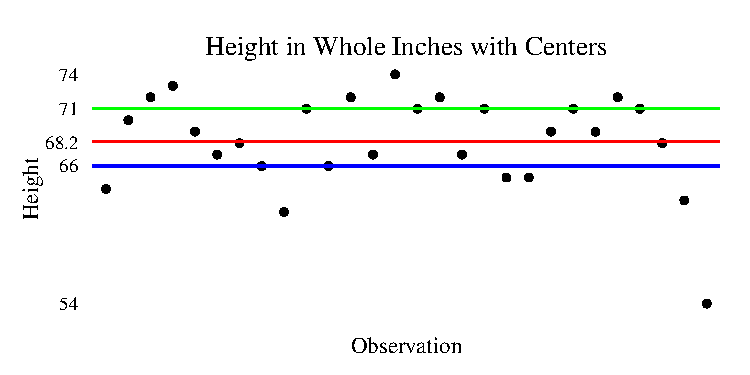
\includegraphics[width=\maxwidth]{figure/graphics-center-chart-1} 

}

\caption[Heights in Observation order with Mode (Green), Median (Blue) and Mean (Red) lines]{Heights in Observation order with Mode (Green), Median (Blue) and Mean (Red) lines}\label{fig:center-chart}
\end{figure}


\end{knitrout}



\section{Measures of Spread}

The ``spread'' of the distribution of a dataset can be quantified by range, first and third quartiles, variance and standard deviation.

We would like to measure the \textbf{Deviation}\marginnote{The \textbf{Deviation} is the  amount by which a single measurement differs from a fixed value, such as the mean.} from the mean. The deviations from the mean are both positive and negative.
\begin{equation*}
Dev_{\bar{x}}=(x_i-\bar{x}) 
\end{equation*}


\begin{knitrout}
\definecolor{shadecolor}{rgb}{0.969, 0.969, 0.969}\color{fgcolor}

{\centering 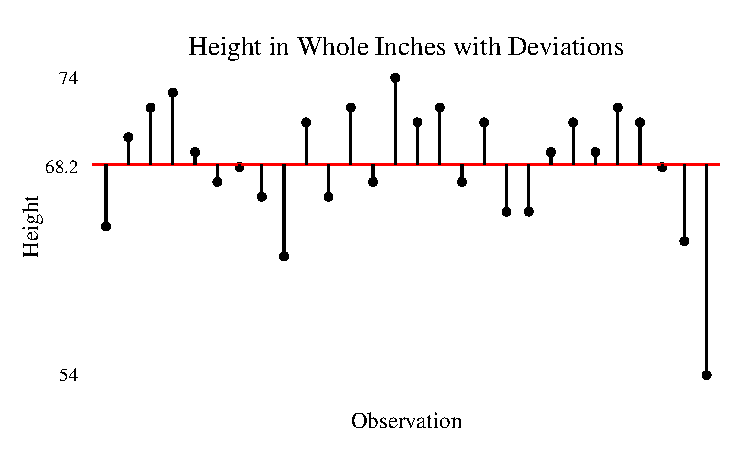
\includegraphics[width=\maxwidth]{figure/graphics-mean-center-chart-1} 

}



\end{knitrout}

The deviations are both positive and negative, and the sum of the deviations is zero, so this statistic alone is not suitable for further analysis. If we square the deviations, the sum is no longer zero; in fact, the sum of the squared deviations is the \textbf{Variance}\marginnote{The \textbf{Variance} is a measure of variability or spread $Var(X)$, often denoted by $\sigma^2$}. The variance of our dataset is 10.39158 square inches. To get back to our original unit of inches, we take the square root of the variance, 3.2, or \textbf{Standard Deviation}\marginnote{The \textbf{Standard Deviation} of X, $StdDev(X)$, often denoted $\sigma$, is the standard measure of spread used in statistical analysis.}
\begin{equation*}
Dev_{\bar{x}}^2=(x_i-\bar{x})^2 
\end{equation*}

\begin{multline*}
Var(X)=\frac{\sum_{i=1}^{N} Dev_{\bar{x}}^2}{N}=\frac{\sum_{i=1}^{N} (x_i-\bar{x})^2}{N}
\end{multline*}

\begin{equation*}
StdDev(X)=\sqrt{Var(X)} 
\end{equation*}

% latex table generated in R 3.1.2 by xtable 1.7-4 package
% Thu Feb 12 10:10:32 2015
\begin{table}[ht]
\centering
\begin{tabular}{lrrr}
  \toprule
Observation & Height & $\dev{x}$ & ${\dev{x}}^2$ \\ 
  \midrule
$x_{1}$ & 64 & -4.5 & 20.6 \\ 
   \rowcolor[gray]{0.95}$x_{2}$ & 70 & 1.5 & 2.1 \\ 
  $x_{3}$ & 72 & 3.5 & 12.0 \\ 
   \rowcolor[gray]{0.95}$x_{4}$ & 73 & 4.5 & 19.9 \\ 
  $x_{5}$ & 69 & 0.5 & 0.2 \\ 
   \rowcolor[gray]{0.95}$x_{6}$ & 67 & -1.5 & 2.4 \\ 
  $x_{7}$ & 68 & -0.5 & 0.3 \\ 
   \rowcolor[gray]{0.95}$x_{8}$ & 66 & -2.5 & 6.4 \\ 
  $x_{9}$ & 62 & -6.5 & 42.7 \\ 
   \rowcolor[gray]{0.95}$x_{10}$ & 71 & 2.5 & 6.1 \\ 
  $x_{11}$ & 66 & -2.5 & 6.4 \\ 
   \rowcolor[gray]{0.95}$x_{12}$ & 72 & 3.5 & 12.0 \\ 
  $x_{13}$ & 67 & -1.5 & 2.4 \\ 
   \rowcolor[gray]{0.95}$x_{14}$ & 74 & 5.5 & 29.9 \\ 
  $x_{15}$ & 71 & 2.5 & 6.1 \\ 
   \rowcolor[gray]{0.95}$x_{16}$ & 72 & 3.5 & 12.0 \\ 
  $x_{17}$ & 67 & -1.5 & 2.4 \\ 
   \rowcolor[gray]{0.95}$x_{18}$ & 71 & 2.5 & 6.1 \\ 
  $x_{19}$ & 65 & -3.5 & 12.5 \\ 
   \rowcolor[gray]{0.95}$x_{20}$ & 65 & -3.5 & 12.5 \\ 
  $x_{21}$ & 69 & 0.5 & 0.2 \\ 
   \rowcolor[gray]{0.95}$x_{22}$ & 71 & 2.5 & 6.1 \\ 
  $x_{23}$ & 69 & 0.5 & 0.2 \\ 
   \rowcolor[gray]{0.95}$x_{24}$ & 72 & 3.5 & 12.0 \\ 
  $x_{25}$ & 71 & 2.5 & 6.1 \\ 
   \rowcolor[gray]{0.95}$x_{26}$ & 68 & -0.5 & 0.3 \\ 
  $x_{27}$ & 63 & -5.5 & 30.6 \\ 
   \rowcolor[gray]{0.95}$x_{28}$ & 64 & -4.5 & 20.6 \\ 
   \bottomrule
Total & 1919.0 &  0.0 & 291.0 \\ 
\rowcolor[gray]{0.95}Total/N & 68.5 &  0.0 & 10.4 \\ 
 & Mean & Zero & Variance \\
\end{tabular}
\caption{Deviations} 
\end{table}


The first and third quantiles can be found by examining either the sorted values or the frequency table, and taking the value of the observation at the first quarter and last quarter. For $n$ observations, the first quartile is the value $(n+1)/4$th entry and the third quartile is the value at the $(n+1)*3/4$th entry, and similar to median, the second quartile, if the calculated entry value is not a whole number, the arithmetic mean of the nearest two observation values determines the mean.



In our height dataset of 28, the first quartile is the 7th observation, 66, and the third quartile is the 21th observation, 71.
\begin{knitrout}
\definecolor{shadecolor}{rgb}{0.969, 0.969, 0.969}\color{fgcolor}\begin{kframe}
\begin{verbatim}
62 63 64 64 65 65 66
66 67 67 67 68 68 69
69 69 70 71 71 71 71
71 72 72 72 72 73 74
\end{verbatim}
\end{kframe}
\end{knitrout}


\section{Distribution Shapes: Histograms, Frequency Polygons, and Ogives}

Once we have calculated the frequencies and centers of our datasets we can start to explore the shape and spread of the distribution of values with charts. All charts can be drawn from the frequency table data.

The \textbf{histogram}\marginnote{A \textbf{Histogram} is a visualization of a frequency table.} is a view of the overall pattern of the distribution. Histogram bars are evenly sized and each bar represents the same class levels of values, and is centered on the mean of the class. The height of the bar represents the number of observations in that class.

The mode can easily be seen on a histogram, and the median is the vertical line at which there is equal area to the left and to the right in the chart. 

A histogram's shape can be symmetric, skewed right with more of the observations on the right or higher values, or skewed to the left with more of the observations on the left or lower values.

A frequency polygon simply displays the frequency for a class, and an ogive, or cumulative frequency polygon displays the cumulative frequency for a class. 

\begin{knitrout}
\definecolor{shadecolor}{rgb}{0.969, 0.969, 0.969}\color{fgcolor}\begin{figure}[h!]

{\centering 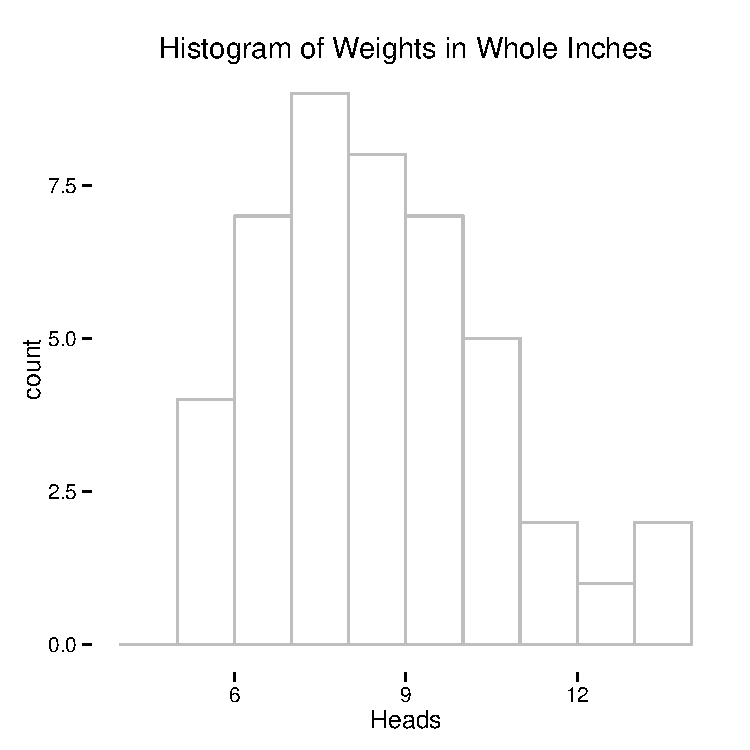
\includegraphics[width=\maxwidth]{figure/graphics-histogram-1} 

}

\caption[Histogram with Frequency Polygon]{Histogram with Frequency Polygon. The Height data set is unimodal, skewed right, with out outlier on the left. }\label{fig:histogram}
\end{figure}


\end{knitrout}


The Empirical Cumulative Distribution shows the possible values of the variable, ordered with frequency, with the cumulative frequency. The proportion of cumulative frequency, often expressed as a percentage, is the number of observations that are less than or equal to the value.

The five number summary of a set of data are the 0th, 25th, 50th, 75th and 100the percentile.

\begin{knitrout}
\definecolor{shadecolor}{rgb}{0.969, 0.969, 0.969}\color{fgcolor}\begin{figure}[h!]

{\centering 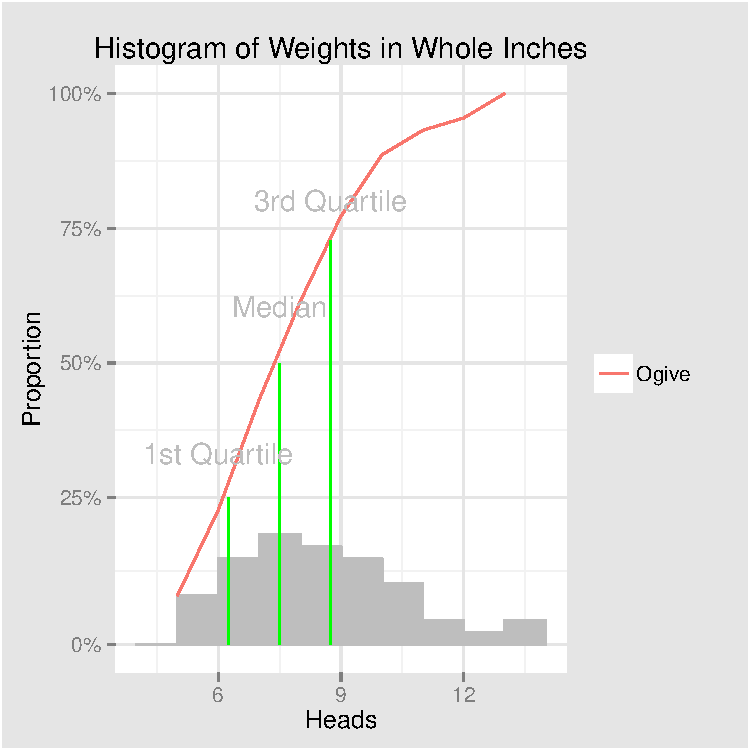
\includegraphics[width=\maxwidth]{figure/graphics-ogive-1} 

}

\caption[Histogram with Ogive (Cumulative Frequency Polygon)]{Histogram with Ogive (Cumulative Frequency Polygon).}\label{fig:ogive}
\end{figure}


\end{knitrout}

The standard deviation, mean and quartiles are used to create a \textbf{boxplot}.

\begin{knitrout}
\definecolor{shadecolor}{rgb}{0.969, 0.969, 0.969}\color{fgcolor}\begin{figure}[h!]

{\centering 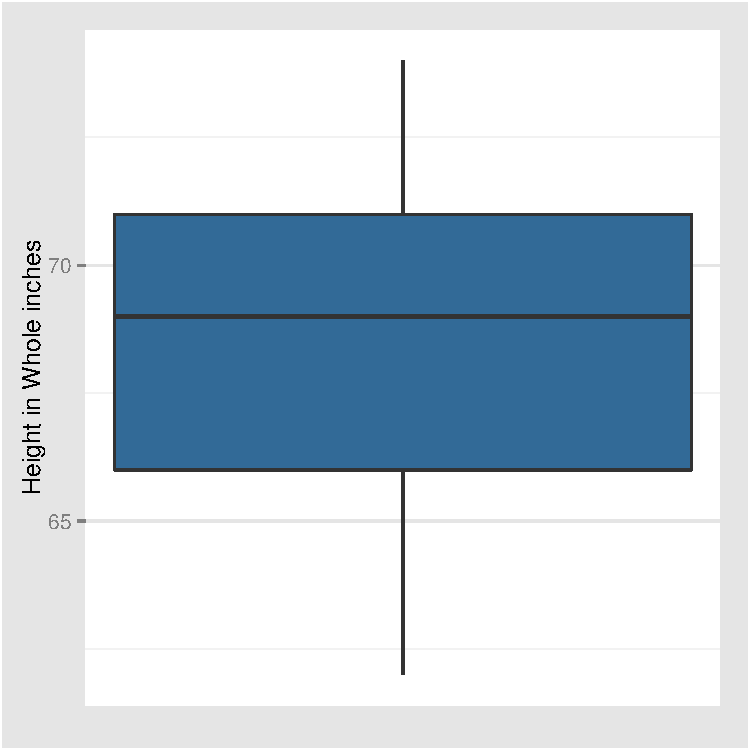
\includegraphics[width=\maxwidth]{figure/graphics-boxplot-1} 

}

\caption[Boxplot]{Boxplot}\label{fig:boxplot}
\end{figure}


\end{knitrout}

\end{document}
